\documentclass[times, 10pt, onecolumn]{article} 
%\documentclass[times, 10pt]{article} 
%\documentclass[conference,final]{IEEEtran}
%\documentclass{article} 

\usepackage{latex8}
\usepackage{times}

%\documentstyle[times,art10,twocolumn,latex8]{article}

%------------------------------------------------------------------------- 
% take the % away on next line to produce the final camera-ready version 
%\pagestyle{empty}

\usepackage[utf8]{inputenc}
\usepackage{graphicx}
\usepackage{url}
\usepackage{float}
\usepackage{times}    
\usepackage{multirow}    
\usepackage{listings}   
\usepackage{times}     
\usepackage{paralist}    
\usepackage{wrapfig}    
\usepackage[small,it]{caption}
\usepackage{multirow}
\usepackage{ifpdf}


\usepackage{listings}
\usepackage{keyval}  
\usepackage{color}
\definecolor{listinggray}{gray}{0.95}
\definecolor{darkgray}{gray}{0.7}
\definecolor{commentgreen}{rgb}{0, 0.4, 0}
\definecolor{darkblue}{rgb}{0, 0, 0.4}
\definecolor{middleblue}{rgb}{0, 0, 0.7}
\definecolor{darkred}{rgb}{0.4, 0, 0}
\definecolor{brown}{rgb}{0.5, 0.5, 0}

\lstdefinestyle{myListing}{
  frame=single,   
  backgroundcolor=\color{listinggray},  
  %float=t,
  language=C,       
  basicstyle=\ttfamily \footnotesize,
  breakautoindent=true,
  breaklines=true
  tabsize=2,
  captionpos=b,  
  aboveskip=0em,
  belowskip=-2em,
  %numbers=left, 
  %numberstyle=\tiny
}      

\lstdefinestyle{myPythonListing}{
  frame=single,   
  backgroundcolor=\color{listinggray},  
  %float=t,
  language=Python,       
  basicstyle=\ttfamily \footnotesize,
  breakautoindent=true,
  breaklines=true
  tabsize=2,
  captionpos=b,  
  %numbers=left, 
  %numberstyle=\tiny
}

\newcommand{\up}{\vspace*{-1em}}
\newcommand{\upp}{\vspace*{-0.5em}}


\title{
  ~\\[-3em]
  Developing Loosely Coupled Applications for Distributed
  Environments using a Standard Programmatic Interface}

  \author{
    ~\\[-2em]
    % Unsure of Author List$^{1}$ \\
    Shantenu Jha$^{1,2,3}$, Joohyun Kim$^{1}$,
    Yaakoub El-Khamra$^{1}$, Andre Merzky$^{1}$ and Hartmut Kaiser$^{1}$\\
    \small{\emph{$^{1}$Center for Computation \& Technology, Louisiana State University, USA}}\\
    \small{\emph{$^{2}$Department of Computer Science, Louisiana State
        University, USA}}\\
    \small{\emph{$^{3}$e-Science Institute, Edinburgh, UK}}\\
  }

%\date{}



\def\acknowledgementname{Acknowledgements}

\newenvironment{acknowledgement}%

{\section*{\acknowledgementname}%
\parindent=0pt%
}

\newif\ifdraft
% \drafttrue
\ifdraft
\newcommand{\kimnote}[1]{ {\textcolor{green} { ***JK: #1 }}}
\newcommand{\alnote}[1]{ {\textcolor{blue} { ***AL: #1 }}}
\newcommand{\amnote}[1]{ {\textcolor{magenta} { ***AM: #1 }}}
\newcommand{\jhanote}[1]{ {\textcolor{red} { ***SJ: #1 }}}
\else
\newcommand{\kimnote}[1]{}
\newcommand{\alnote}[1]{}
\newcommand{\amnote}[1]{}
\newcommand{\jhanote}[1]{}
\fi

\begin{document} 


\maketitle    

\begin{abstract}
  The Simple API for Grid Applications (SAGA) can be used to
  programmatically develop a very wide-range of distributed
  applications.  In this paper we describe how SAGA has been used to
  develop two different applications from the following classes of
  distributed applications (i) applications based upon the loosely
  coupled of homogenous sub-tasks and, (ii) applications based upon
  loosely coupled simulations of heterogenous sub-tasks. The specific
  applications developed are Replica-Exchange simulations using
  Molecular Dynamics and Kalman-Filter based application for reservoir
  simulation.  We briefly discuss the specific applications developed
  and the typical science problems tackled using these applications.
  We will describe the application characteristics of the two
  case-studies, with a focus on the distributed logic of these
  simulations, and not the core simulation logic of the applications.
  The paper analyses and contrasts the application characteristics of
  the examples, and shows how they are supported using SAGA, often in
  conjunction with other programming frameworks such as Cactus.  The
  primary aim of this paper is to demonstrate how SAGA can be an
  effective tool for programmatically representing and implemeting the
  logic of coordination and orchestrating multiple, distributed tasks,
  while remaining agnostic to the actual mechanism, ie. details of the
  distributed environment. We will highlight the importance of
  programming abstractions and how frameworks that provide common
  programming patterns can be used to simplify the construction of
  distributed applications.


\end{abstract}

% \Section{Introduction}
%   There exist several applications which require several smaller but
%   heterogenous tasks to be solved in multiple-stages as part of the
%   overall solution.  Often the time-to-solution is the single most
%   important metric.  Distributed resources can thus help, especially
%   when combined with opportunistic scheduling/execution.  However, the
%   desire/need to use distributed computing comes with its own/unique
%   set of challenges.
  
%   We discuss three application types that are in turn composed of
%   multiple, smaller but {\it loosely-coupled} tasks -- Replica
%   Dynamics, Satisfiability problems, and Kalman filtering
%   applications.  Although these applications types are similar in that
%   they are comprised of multiple, smaller tasks, they are different in
%   that the individual sub-tasks are dissimilar for different reasons.
  
%   These application types are often multi-staged, with varying levels
%   of dependency between the stages. There could be, strict ordering
%   between the stages, ie. if all tasks in a stage must complete and be
%   globally synchronised before the next stage can begin. Thus there is
%   coupling between tasks within a given stage, and there is coupling
%   between stages.

%   Other challenges that any many-task system will encounter are: (i)
%   scheduling these sub-tasks is a challenge, (ii) level of speculative
%   computing that can be employed.

%   In parallel replica dynamics, the replicas can run for different
%   time durations between different stages. In replica-exchange
%   dynamics, the number and frequency of exchanges can vary.  Different
%   stages of this application vary; in other words, there is
%   time-domain heterogenity.

%   In Kalman filter based applications, the number and size of 
%   tasks between different stages varies. 

%   In the general class of satisfiability-based applications, as well
%   as the learning-based algorithms, there are elements of both kinds
%   of heterogenity between stages. GridSAT is an interesting example.
                           

% \begin{acknowledgement}
%   \up This work would not have been possible without the efforts and
%   support of the wider SAGA team, especially Hartmut Kaiser, Ole
%   Weidner and Joao Abecasis. Important funding for SAGA specification
%   and development has been provided by the UK EPSRC grant number
%   GR/D0766171/1 (via OMII).  SJ acknowledges the e-Science Institute,
%   Edinburgh for supporting the research theme, ``Distributed
%   Programming Abstractions''.  This work has also been made possible
%   thanks to the internal resources of the Center for Computation \&
%   Technology (CCT) at Louisiana State University and computer
%   resources provided by LONI.
% \end{acknowledgement}


\bibliographystyle{IEEEtran}
\bibliography{saga}
\end{document}


%Migol provides an integrated solution for the management of data and
%compute resources.

% A main limitation of current Grid infrastructures is the restricted availability of 
% precise resource information. Managing this information uncertainty is difficult and often leads to
% a trial-and-error approach. For example, a transfer service cannot 
% differentiate between a harddisk failure and a transient network failure. While a retry 
% will resolve a transient failure, in case of a harddisk failure this approach will very likely not be successful.
% An adaptive strategy for tuning fault detection timeouts is therefore essential to achieve a 
% sufficient reliable fault detection while maintaining an acceptable performance.        

% Granularity of SAGA API not always well suited for Grid service interactions.
%%------------------------------------------------------------------------------     




% \begin{abstract}   {Grid Computing, Task Farming, SAGA, Migol}
% A major challenge in a dynamic Grid with thousands of machines connected to
% each other is fault tolerance. The more resources and components involved, the
% more complicated and error-prone becomes the system. 
% Migol~\cite{schnorLuckow08} is an adaptive Grid middleware,
% which addresses the fault tolerance of Grid applications and services 
% by providing the capability to recover applications from checkpoint files 
% transparently. 
% 
% SAGA~\cite{SAGA_Goodale06a} provides a standardized, application-level API for 
% common Grid scenarios, e.\,g.\
% the management of files and jobs. The new SAGA Checkpoint Recovery (CPR) package addresses checkpointing 
% and the automatic recovery of Grid applications. In this paper, we describe the design of 
% the SAGA-CPR package, the integration of the CPR adaptor with the Migol infrastructure, 
% and our experiences with running a large scale SAGA-CPR based task farming application 
% in a real Grid environment. 
% \end{abstract}   

%%------------------------------------------------------------------------------
% Open Topics:
% How long running are Map-Reduce sorting problems?
% Sorting with MapReduce: 1TB data => runtime 891 s (Dean, Google)
% SAGA provides a more low level primitives than Hadoop or Google MapReduce.
% What failure detection timeouts per task should be used?
% Performance measurement: without versus with failures    
% Comparison w/ Google MapReduce infrastructure:
%         - Master responsible for allocating mapper tasks (close to data)   
% Limitations of SAGA map-reduce
%       - low-level handling of file transfers and jobs required (ft aspect can be handled by Migol) 
%       - no sorting of data between map and reduce



% Long-running applications can significantly benefit from Migol:
% Without human interaction, recovery times are minimized, and the
% application and infrastructure utilization is enhanced.  While the
% Google's map-reduce infrastructure is tailored to the special needs
% of Google, SAGA provides an open standard, which allows the
% middleware independent implementation of MapReduce. Migol can
% provide a fault-tolerant run-time for map and reduction tasks
% handling resource allocation across VOs, staging, starting and
% re-starting of tasks transparently.
 
% Fault tolerance important:
% - One empty fail or the failure of a mapper task should not mess up the entire computation
% - if a particular input does not work - infrastructure will eventually give up
% - no reduce can start until map is complete - a single slow disk controller can rate-limte the whole process
% - master can re-execute slow-moving tasks redundantly (use results who first finishs)
% - mapreduce factors out synchronization
% - Reduce phase cannot start until all map tasks finished, i.\,e.\ it is not possible to achieve a result unless all 
% tasks have been finished.



% This paper is structured as follows: after an overview about related work 
% in section~\ref{sec:related} and the Migol service framework in 
% section~\ref{sec:migol}, this paper describes in detail the design of the 
% Checkpoint Recovery API for SAGA as well as the 
% the Migol adaptor. In section~\ref{sec:exp} we present our experiences 
% with checkpoint recovery of a task farming application in the 
% LONI~\cite{Allen:2003xy} Grid environment.      
   

%%------------------------------------------------------------------------------

% The objective of SAGA-CPR is to mostly hide the complexity of a
% GridCPR infrastructure, such as making calls to different
% infrastructure services for registering information etc., from the
% application developer. Most interactions are handled transparently
% within the adaptor.  The SAGA-CPR package provides a generic,
% middleware-independent API to a GridCPR middleware.
    
% For the management of checkpoint metadata the SAGA-CPR API use the
% namespace paradigm to hierarchically organize files and directories.
% Checkpoint directories are used to group checkpoints. Parallel
% applications often write one checkpoint per processor, i.\,e.\ in
% case of $n$ processors a CPR checkpoint would consists of $n$ files.
% Thus, a CPR checkpoint is designed as container for multiple
% physical or logical files.
% 
%                                                       
% For execution and management of CPR jobs, SAGA defines a CPR job.
% The management of CPR jobs is similar to regular jobs: A job is
% defined by a job description. In contrast to normal jobs, CPR jobs
% require two job descriptions -- one for starting and another one for
% restarting the application.  Jobs are started using the job service.
% In addition to the normal job controls, a CPR job can be queried for
% checkpoint metadata, and it can be explicitly checkpointed or
% recovered.
% 
% In general, fault detection is done by a monitor process, which
% periodically sends keep-alive messages to applications.  Since the
% remote monitoring capability for applications can be completely
% hidden within the SAGA adaptor no explicit API is required. The SAGA
% adaptor can transparently start a monitoring endpoint without
% requiring any user interaction.  In case a SAGA application does not
% respond to a heartbeat message for a certain time a recovery is
% initiated by the Grid middleware, e.\,g.\ by Migol's MRS.

% Remote steering of SAGA applications can be implemented using the
% SAGA Monitorable API in conjunction with the job self object.

% With the described functionality the SAGA-CPR package is well suited to 
% provide a clean abstraction to the Migol middleware. 
% Of course, the package can also be facilitated by another middleware adaptor. 
% In the following the Migol SAGA adaptor is described.   

% \subsection{SAGA-CPR Migol Adaptor}
% 
% Currently, a C++ and Java implementation for SAGA exists. Although the Migol backend mainly consists 
% of web services Migol especially addresses the fault tolerance of long running e-Science applications written
% in C/C++. These  computing intensive applications have high performance requirements and, in general, require 
% native libraries, e.\,g.\ for numerically computations, or MPI for cluster communication. Thus, we focus on the 
% SAGA C++ reference implementation~\cite{Kaiser:2006qp}. 
% 
% % SAGA enables a seamless integration of an application into the Grid while Migol provides infrastructure 
% % services, such as monitoring, resource reservation and allocation. For example, an application 
% % can initiate a migration in case it detects a failure using the SAGA API. Migol will then be 
% % migrated e.\,g.\ it allows the application to start an migration in case it detects a 
% % failure or a performance bottleneck.  
% 
% \begin{figure}[t]
%   \centering
%   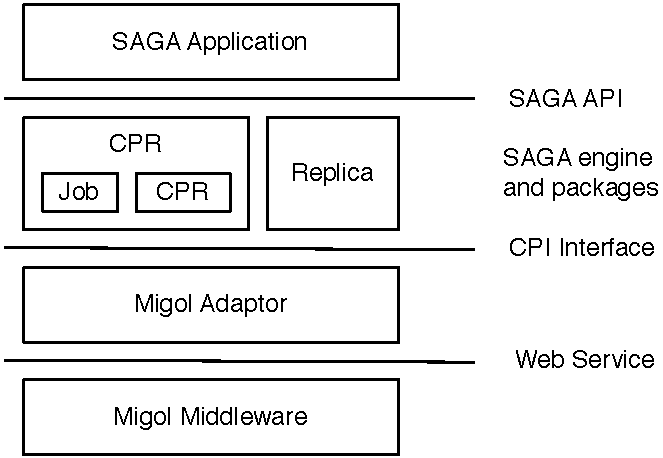
\includegraphics[width=0.6\textwidth]{saga-migol-layered}
%   \caption{\footnotesize \bf SAGA Adaptor for Migol infrastructure}
%   \label{fig:saga-migol-layered}
% \end{figure}  


% \section{Experiences with a Large-Scale Task-Farming Application in the LONI Grid}
% \label{sec:exp}       
% 
%         
% %do we use checkpoints or do we automatically restart the task
% Figure~\ref{fig:saga-taskfarming} gives an overview about the task farming scenario. All tasks are
% distributed using a script and Migol's Job Broker Service.
% %  Each worker will compute a certain 
% % variation of the graph network. Depending on the graph size, the runtime of a single task  can 
% % be as high as \textbf{TODO}  days. 
% To enable the monitoring of a tasks, each task must initialize a \texttt{saga::session} object 
% before starting the computation.  Then, the Migol adaptor starts and registers the monitoring endpoint. 
% %TODO what is the task size/runtime of a single task
% The MRS can now monitor the application.  For error detection we use a timeout of 5 minutes.
% \begin{figure}[t]
%     \centering
%         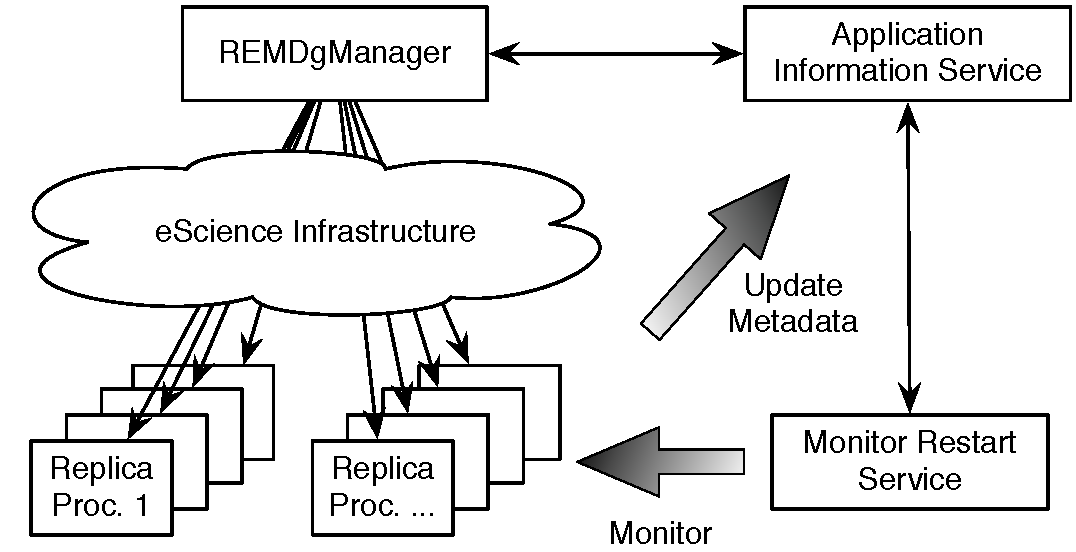
\includegraphics[width=\textwidth]{saga-taskfarming}
%     \caption{\footnotesize \bf Fault-Tolerant Task Farming Scenario}
%     \label{fig:saga-taskfarming}
% \end{figure}
% 
% 
% 
% 
%   
% 
% During the runtime, we simulate the failure of a number of worker
% processes.  The Migol MRS successfully detects the respective faults
% and recovers the worker nodes correctly. Even with a high failure
% rate, we were able to obtain the results of our computation.

